\documentclass[11pt, journal, onecolumn]{IEEEtran}

\usepackage{amsmath, amssymb, amsthm, mathtools, bm}
\newtheorem{lemma}{引理}
\newtheorem{theorem}{定理}
\newtheorem{proposition}{命题}
\usepackage{booktabs, array, tabularx, multirow, makecell, colortbl}
\usepackage{graphicx}
\graphicspath{{figuras/}}
\usepackage{tikz}
\usetikzlibrary{arrows.meta, positioning, calc, shapes.geometric}
\usepackage{algorithm}
\usepackage{algpseudocode}
\usepackage{cite}
\usepackage{xeCJK}
\setCJKmainfont{Noto Serif CJK SC}
\setCJKsansfont{Noto Sans CJK SC}
\setCJKmonofont{Noto Sans Mono CJK SC}
\usepackage{hyperref}
\hypersetup{colorlinks=true, linkcolor=blue, citecolor=blue, urlcolor=blue}

%% Cabeceras de clase en idioma nativo (adenda menor de cierre pulcro)
\renewcommand\abstractname{摘要}
\renewcommand\IEEEkeywordsname{关键词}

%% --- Paleta cromática institucional SENI-IA ---
\definecolor{seni-blue}{RGB}{0,45,98}
\definecolor{seni-red}{RGB}{206,17,38}
\definecolor{seni-gold}{RGB}{201,168,76}
\definecolor{seni-green}{RGB}{0,122,51}
\definecolor{seni-dark}{RGB}{26,26,26}

%% ====================================================================
%% EDICIÓN EN CHINO MANDARÍN (1 columna, xeCJK/xelatex)
%% El texto canónico internacional es la edición inglesa.
\title{SENI-142：依据第368-22号领土规划法实施对角分块划分的多米尼加共和国开放、高韧性岛屿输电基准}

\author{Junior~Alexis~Villanueva-Rosario,~\IEEEmembership{Ms.C., Ph.D.(c)}\\[0.3em]
{\normalsize\textnormal{\textbf{V-TECH} \textbar\ \textbf{V-CORE TECH S.R.L.} / \textbf{Villa-Core Technologies, S.L.}}}\\[0.15em]
{\footnotesize\textnormal{\textit{Department of Electrical Grids and Renewable Energy (EERR) Research}}}\\[0.15em]
{\footnotesize\textnormal{\textit{电力系统与人工智能博士讲席（Doctoral Chair）}}}\\[0.15em]
{\footnotesize\textnormal{多米尼加共和国圣多明各 \textbar\ \texttt{ingjavillanueva@gmail.com}}}%
\thanks{J. A. Villanueva-Rosario 任职于 Department of Electrical Grids and Renewable Energy (EERR) Research, V-TECH (V-CORE TECH S.R.L. / Villa-Core Technologies, S.L.)，多米尼加共和国圣多明各（电子邮箱：ingjavillanueva@gmail.com）。}}

% --- Optimización de ubicación de figuras y tablas flotantes ---
\renewcommand{\topfraction}{0.95}
\renewcommand{\bottomfraction}{0.95}
\renewcommand{\textfraction}{0.05}
\renewcommand{\floatpagefraction}{0.8}
\renewcommand{\dbltopfraction}{0.95}
\renewcommand{\dblfloatpagefraction}{0.8}
\setcounter{topnumber}{4}
\setcounter{bottomnumber}{2}
\setcounter{totalnumber}{6}
\setcounter{dbltopnumber}{4}

\begin{document}
\maketitle

\begin{abstract}
孤立电力系统是能源转型中最严苛的试验场：它们无法输入惯量、旋备或邻网支援，而多米尼加共和国近期经历的全国性停电已在全国尺度上暴露了这种脆弱性。本文贡献\textbf{SENI-142}：一个覆盖整个加勒比国家输电网络的开放、全面地理配准的基准——多米尼加共和国142节点互联系统（SENI），包含约112座物理变电站、135条输电线路与58台电力变压器，横跨345、230与138~kV电压层，辐射状69~kV配电层经等效多端口化简。该基准按国家领土规划法令（第368-22号法律）划分为十个主权领土微电网，并以分层边界-坐标列式（HBCF）凝聚，其精确舒尔补凝聚在消费级硬件上以\textbf{2.65~ms}、\textbf{473~MiB}常驻内存求解完整国家电网的每个小时级交流状态，相量边界耦合残差为 $\delta = 2.788 \times 10^{-14}$~pu。结构求解器以87,360个连续运行小时（2016--2025年）的真实系统运营商遥测、经保持日间气候相关性的24小时块自助法进行校准与验证，并以215个预想事故的 $N-1$ 目录进行压力测试。87,360状态的多时段算例与215项预想事故筛选均出自作者已申请专利（patent-pending）的C++/稀疏引擎；公开发布的数据包认证的是网络模型、凝聚求解不变量与八项典型预想事故的功率平衡。确定性的四相数字孪生生命周期——密封飞地、动态科研测试台压测、SHA-512黄金主版本、原子化内核晋升——使每项报告数字逐位可复现。多向量灵活性（电转气氢能、764~MW可逆抽蓄、ADM1生物甲烷化）耦合到多时段AC-OPF，并以分区CAPEX/OPEX证明加以验证。数据集、拓扑与验证工具经IEEE DataPort与GitHub开放发布。
\end{abstract}

\begin{IEEEkeywords}
AC最优潮流，数字孪生，储能，孤立电力系统，节点导纳矩阵，氢能，网络分块（diakoptics），区间微电网划分，舒尔补，输电网络，弹性电力系统，领土空间规划。
\end{IEEEkeywords}

% =========================================================================
% secciones_zh/sec01_introduction.tex — 第I节，中文版（精修版）
% =========================================================================
\section{引言}
\label{sec:intro}

孤立互联电网处于电力工程设计空间的极端位置。岛屿无法从邻近电网输入惯量、无功支撑或紧急输送功率：每一兆瓦的备用容量、每一伏安的无功补偿和每一兆赫的阻尼能力，都必须在消费它的同一同步覆盖区内生产、调度和防御。多米尼加共和国是一个典型案例：一个约有一千一百万人口的单一同步岛，无海底或陆上互联，全国百分之四十以上的负荷集中在奥萨马（Ozama）都市区，惯量锚点由蓬塔卡塔利纳（Punta Catalina）燃煤电厂主导，且可再生能源建设的瞬时光伏渗透率在运行遥测中已达到需求的36.6\%\cite{ocseni}。失去发电--负荷平衡所造成的全国性后果并非假设：2025年11月与2026年2月记录在案的全国性停电事件\cite{ocseni}曾以整个领土的规模动员应急响应，并重新引发了关于频率稳定性、黑启动能力与输电资产可观测性的公共政策辩论\cite{blackout2004}。这种脆弱性的物理机理如今已是经典\cite{kundur1994}——系统惯量下降会劣化频率变化率并收窄变流器主导电网的可控包络\cite{tielens2016}、\cite{milano2018}、\cite{dorfler2013}、\cite{hatziargyriou2021}——但可用于研究它的实证工具仍然出奇地原始。

本领域的基准测试基础设施大多是合成的。至今仍主导博士训练与对比研究的经典测试系统——WSCC 9节点系统以及IEEE 14、30、57、118节点系统——都源自二十世纪六十年代初的制图台式抽象：电抗是圆整的学术数字，负荷是固定的功率三角形，没有地理，没有气候，数据集中没有任何元件曾跳闸、检修、付费或遭受过飓风。另一个极端上，电力公司级的电网案例保存在商业仿真平台的专有格式中，受保密约束，很少以允许独立重新执行的形态发布。开源运动提供了宝贵的基础设施——MATPOWER算例库\cite{matpower2011}与AC-OPF基准算例的电力网格库（Power Grid Library）\cite{pglib2019}等——但其算例几乎无一例外是\emph{合成或匿名的}：它们是为"难"而生的电网，而不是真实存在的电网。在玩具与机密之间几乎一无所有：一个开放的、完整的、实测的真实国家输电系统模型，其溯源性足以支持独立验证——这是加勒比海岛屿世界（乃至整个岛屿世界）当前所缺乏的公共品。

本文以\textbf{SENI-142}弥合这一鸿沟：一个围绕三项承诺构建的开放基准。第一，\textbf{对实测现实的忠实}：网络模型不是合成的——它源自国家输电资产，并以87,360个连续运行小时（2016--2025年）的系统运营商遥测数据逐机组、逐小时地进行验证，使每个仿真状态都对应一个存档的运行状态。第二，\textbf{对尺度的结构诚实}：求解的是全国完整系统——全部输电母线、全部干线、全部变压器——而非其缩减片区，且求解方法以定理而非愿望的形式给出其精确性与复杂度：网络分块（diakoptics）传统\cite{kron1963}、\cite{happ1971}下的分层边界-坐标列式（HBCF），经舒尔补\cite{zhang2005}凝聚，并在国家领土规划法（第368-22号法律）\cite{ley368}规定的十个领土规划区上分解因式。第三，\textbf{确定性可复现}：每个工件都通过具有失效即闭（fail-closed）校验门级联、SHA-512分离式封存与原子化晋升的四阶段数字孪生生命周期，使本文报告的任何数字都可以从逐位相同、经密码学证明的软件状态重新生成。

贡献有五项，且每项均可证伪：
\begin{itemize}
\item \textbf{C1 —— 基准。}多米尼加共和国完整输电网络的开放、地理配准、符合标准的模型：约112座物理变电站之上的142个节点，135条输电线路，58台电力变压器，345、230与138~kV三个电压层，69~kV subtransmission层经保持注入的等效化简；随附拓扑、参数、溯源性元数据与验证工具，通过IEEE DataPort与GitHub开放发布。
\item \textbf{C2 —— 列式。}将完整岛屿电网网络分块划分为十个主权领土微电网——即第368-22号法律的规划区——并聚合为四个电气宏域、边界集最小的HBCF划分，以及其舒尔补凝聚的精确性证明：复杂度 $O(\sum_k N_k^3 + N_B^3)$，对比整体稠密分解的 $O(N^3)$。
\item \textbf{C3 —— 确定性数字孪生。}四阶段生命周期（带十四道失效即闭校验门级联的POSIX命名空间密封飞地；针对215个预想事故目录的动态科研测试台 $N-1$ 压力测试；SHA-512分离式封存的黄金主版本；经 \texttt{renameat2} 的原子化内核晋升，回归量为零），将以链式凭证把仿真遥测转化为证据。
\item \textbf{C4 —— 多向量灵活性。}将电转气氢能（电解、700~bar存储、燃料电池再注入）、764~MW可逆抽水蓄能与基于ADM1的生物甲烷化耦合到多时段AC-OPF，给出完整的Karush--Kuhn--Tucker（KKT）条件体系，并以分区CAPEX/OPEX平衡证明加以验证。
\item \textbf{C5 —— 实测硅上性能。}在消费级硬件上以2.65~ms、473~MiB常驻内存与 $\delta = 6.35 \times 10^{-12}$~pu 的相量边界残差求解每个全国小时级交流状态——快于60~Hz下8.33~ms的半周期实时阈值——并采用24小时块自助法验证协议。
\end{itemize}

本文余下部分的组织如下。第~\ref{sec:methodology}节阐述方法论：不变列式（图模型、69~kV化简、HBCF划分、舒尔补凝聚、数据协议、确定性生命周期、无功限值正则化、多时段AC-OPF）与在多米尼加案例上按第368-22号法律实例化的领土条款。第~\ref{sec:topology}节记录基准拓扑：从112座变电站的物理资产到142节点模型与十个领土微电网。第~\ref{sec:multivector}节展开多向量灵活性星座及其分区经济性验证。第~\ref{sec:benchmarking}节报告硅上性能、精度与预想事故韧性。第~\ref{sec:discussion}节讨论政策启示与局限，第~\ref{sec:conclusion}节以开放发布计划与四条研究路线作结。

% =========================================================================
% secciones_zh/sec02_methodology_seni_ia.tex — 第II节，中文版（精修版）
% =========================================================================
\section{方法论：HBCF网络分块舒尔补列式与失效即闭数字孪生生命周期}
\label{sec:methodology}

该方法有意组织为两个耦合组件。\textbf{不变列式}——图表示、等效化简、空间划分、精确凝聚、数据协议、确定性生命周期、正则化与优化——与问题无关，可在本平台所支撑的整个研究族中不加修改地迁移。\textbf{领土实例化条款}则将该列式绑定到一个参考现实：按国家自身领土规划法令划分的多米尼加共和国国家电网。这种划分并非出于美学：正是它使基准成为一个可复用的科学仪器，而不是一次性的案例研究。

\subsection{输电网的图论表示}
\label{sub:graph}

输电系统建模为连通无向图 $\mathcal{G} = (\mathcal{V}, \mathcal{E})$ \cite{newman2010}，其中 $\mathcal{V}$ 为输电节点集（$|\mathcal{V}| = 142$），$\mathcal{E} = \mathcal{E}_{\mathrm{line}} \cup \mathcal{E}_{\mathrm{trafo}}$ 为线路支路与变压器支路之并，$|\mathcal{E}_{\mathrm{line}}| = 135$ 条输电线、$|\mathcal{E}_{\mathrm{trafo}}| = 58$ 台电力变压器。每条支路在100~MVA公共基值下携带标幺串联导纳与半充电电纳；节点导纳矩阵 $\mathbf{Y}_{\mathrm{bus}} \in \mathbb{C}^{142 \times 142}$ 由此编码了20,164个耦合电磁状态的复数元素。节点功率注入遵循标准直角坐标平衡方程
\begin{equation}
S_i = P_i + jQ_i = V_i \sum_{j \in \mathcal{V}} Y_{ij}^{*}\, V_j^{*}, \qquad i \in \mathcal{V},
\label{eq:balance}
\end{equation}
节点分为平衡节点（slack）、PV节点与PQ节点\cite{tinney1967}。平衡节点职责——设定相位参考并吸收有功失衡——由胡利奥·萨乌里（JSAURI）变电站的345~kV母线承担，电压保持 $V = 1.02$~pu，直接接收全国最大火电厂的注入（第~\ref{sub:strata}节）。凡物理变电站容纳多个电压等级，每个电压等级即为一个独立节点，其间自耦变压器为一条支路；这一统一应用的单一规则，使网络从约112座围栏场站精确升至142个节点（第~\ref{sub:substations}节）。

\subsection{69 kV配电层的等效化简}
\label{sub:reduction}

运行于69~kV的辐射式subtransmission与中压子网络被凝聚为戴维南/诺顿型静态多端口等效。对每个保留的边界端口，等效保持（i）被凝聚区域在每个建模小时的聚合复功率注入，以及（ii）从边界看到的短路阻抗 $Z_{\mathrm{cc}}$（经Kron型网络化简获得）。形式上，对边界端口 $p$ 与被凝聚内部 $\Omega_r$：
\begin{equation}
V_p = E_{\mathrm{th}}^{(r)} - Z_{\mathrm{th}}^{(r)} I_p, \qquad \sum_{i \in \Omega_r} S_i = V_p I_p^{*},
\label{eq:thevenin}
\end{equation}
因此该化简在潮流意义下\emph{在边界处无损}，同时消除了 $\mathbf{Y}_{\mathrm{bus}}$ 的维度膨胀。化简从资产存档配置重新计算，其本身也是封存工件的一部分，符合工业系统分析的推荐实践\cite{ieee399}与基于CIM的电网模型交换\cite{iec61970}。

\subsection{空间网络分块：HBCF}
\label{sub:hbcf}

分层边界-坐标列式（HBCF）将 $\mathcal{G}$ 划分为 $K$ 个两两点不相交的领土子系统 $\mathcal{G}_k = (\mathcal{V}_k, \mathcal{E}_k)$，仅通过最小割边集 $\mathcal{V}_B = \bigcup_{k=1}^{K} \partial \mathcal{V}_k$ 互连。该划分\emph{在两个层级上分层}：
\begin{enumerate}
\item \textbf{法域-领土层级。}国家领土规划法令——第368-22号法律（领土规划、土地利用与定居点法）\cite{ley368}——将全国领土组织为十个规划区。基准采纳这十个区作为其十个主权领土微电网，使电气划分与领土治理重合——一个具有直接政策后果的建模决策（第~\ref{sec:discussion}节）。
\item \textbf{电气层级。}为数值凝聚，十个微电网捆绑为 $K = 4$ 个电气宏域——北部（Cibao）、南部、东部与都市区——其间互连恰为资产的230/138~kV干线联络。边界集 $\mathcal{V}_B$ 即这些联络的关联节点集；对干线支路执行Kron切割\cite{kron1963}、\cite{happ1971}即可隔离各子域并定义凝聚边界 $\Gamma$。
\end{enumerate}

将节点重排为 $(\text{内部} \mid \text{边界})$ 后，任一运行点上的节点雅可比或导纳系统取分块形式
\begin{equation}
\begin{bmatrix} \mathbf{A} & \mathbf{B} \\ \mathbf{C} & \mathbf{D} \end{bmatrix} \begin{bmatrix} \mathbf{x}_I \\ \mathbf{x}_B \end{bmatrix} = \begin{bmatrix} \mathbf{u}_I \\ \mathbf{u}_B \end{bmatrix},
\label{eq:blockform}
\end{equation}
其中 $\mathbf{x}_I$ 收集所有子域的内部变量，$\mathbf{x}_B$ 为边界状态。由构造，$\mathbf{A} = \operatorname{diag}(\mathbf{A}_1, \dots, \mathbf{A}_K)$ 为分块对角阵，$\mathbf{A}_k$ 是宏域 $k$ 的内部雅可比块。

\subsection{舒尔补的精确凝聚}
\label{sub:schur}

凝聚依赖三个初等但影响深远的结果，此处完整陈述，因为它们承载着基准的精确性主张。

\begin{lemma}[分块对角逆]
\label{lem:blockdiag}
若 $\mathbf{A} = \operatorname{diag}(\mathbf{A}_1, \dots, \mathbf{A}_K)$ 且各 $\mathbf{A}_k \in \mathbb{R}^{N_k \times N_k}$ 非奇异，则 $\mathbf{A}^{-1} = \operatorname{diag}(\mathbf{A}_1^{-1}, \dots, \mathbf{A}_K^{-1})$。
\end{lemma}
\begin{proof}
显然：对每个块位置 $(k, l)$，当 $l = k$ 时 $\mathbf{A}_k \mathbf{A}_k^{-1} = \mathbf{I}_{N_k}$，否则 $\mathbf{A}_k \cdot \mathbf{0} = \mathbf{0}$；该乘积在内部空间的直和上等于单位阵。
\end{proof}

\begin{theorem}[舒尔凝聚的精确性]
\label{thm:schur}
若完整系统矩阵 $\begin{psmallmatrix} \mathbf{A} & \mathbf{B} \\ \mathbf{C} & \mathbf{D} \end{psmallmatrix}$ 非奇异且 $\mathbf{A}$ 非奇异，则 $\mathbf{x}_B$ 是如下降阶边界系统的唯一解
\begin{equation}
\mathbf{S}\, \mathbf{x}_B = \mathbf{u}_B - \mathbf{C}\, \mathbf{A}^{-1} \mathbf{u}_I, \qquad \mathbf{S} = \mathbf{D} - \mathbf{C}\, \mathbf{A}^{-1} \mathbf{B},
\label{eq:schur}
\end{equation}
且 $\mathbf{x}_I = \mathbf{A}^{-1}(\mathbf{u}_I - \mathbf{B}\, \mathbf{x}_B)$ 恢复内部状态。二元组 $(\mathbf{x}_I, \mathbf{x}_B)$ 与未降阶分块系统的唯一解重合。
\end{theorem}
\begin{proof}
对完整系统作分块高斯消元：将第一行左乘 $\mathbf{C}\mathbf{A}^{-1}$ 并从第二行减去，消去 $\mathbf{x}_I$，得到上述边界系统；这些是非奇异行变换，故降阶系统与原系统等价，唯一性由非奇异性假设传递。回代即消元的第二行。当且仅当完整矩阵非奇异时，舒尔补 $\mathbf{S}$ 非奇异\cite{zhang2005}。
\end{proof}

\begin{proposition}[复杂度]
\label{prop:complexity}
$N$ 节点系统的稠密分解代价为 $O(N^3)$；分块求解的代价是一次分块对角分解 $\sum_k O(N_k^3)$ 加一次边界分解 $O(N_B^3)$ 加消元乘积，即 $O\!\left(\sum_k N_k^3 + N_B^3\right)$，其中 $\sum_k N_k + N_B = N$ 且 $N_B \ll N$。对经填充降低排序分解的稀疏 $\mathbf{A}_k$，局部代价趋于 $N_k$ 的线性\cite{george1973}、\cite{saad2003}。
\end{proposition}

凝聚的数值治理本身即被测量。边界系统的谱条件数 $\kappa_2$ 在每个运行点被监测\cite{vancutsem1998}；相量重建残差——凝聚恢复状态与参考状态之间的最大失配——在整个验证水平域上实测为 $\delta = 6.35 \times 10^{-12}$~pu。作为外部效度控制，同一谱方法学首先在合成算例上进行了压力校验：例如经典IEEE 14节点系统的 $22\times22$ 雅可比矩阵在项目谱分类中被评为MARGINAL（边缘），$\kappa_2 = 117.7823$，该分类在任何国家级部署之前均经独立工具交叉验证。算法~\ref{alg:schur_pf}给出完整求解器。

% ---- 算法1注入块 ----
\begin{algorithm}[!t]
\caption{SENI-142 HBCF划分上的边界-舒尔交流潮流}
\label{alg:schur_pf}
\begin{algorithmic}[1]
\Require 划分 $\{\mathcal{G}_k\}_{k=1}^{4}$，边界集 $\mathcal{V}_B$，
         小时级注入 $(\mathbf{u}_I, \mathbf{u}_B)$，容差 $\varepsilon$
\Ensure 收敛状态 $(\mathbf{x}_I, \mathbf{x}_B)$，残差 $\rho$
\State 初始化平启动 $(\mathbf{x}_I^{(0)}, \mathbf{x}_B^{(0)})$
\State 组装 $\mathbf{J}^{(0)} = \begin{psmallmatrix} \mathbf{A} & \mathbf{B} \\ \mathbf{C} & \mathbf{D} \end{psmallmatrix}$
\For{$t \gets 0, 1, 2, \dots$ 直至 $\rho \le \varepsilon$}
  \For{$k \gets 1, \dots, K$} \Comment{并行，内存互不相交}
     \State $\mathbf{A}_k^{(t)} \gets \partial (\Delta \mathbf{u}_k) / \partial \mathbf{x}_k$
     \State 以填充降低排序分解 $\mathbf{A}_k^{(t)} = \mathbf{L}_k \mathbf{U}_k$
  \EndFor
  \State $\mathbf{W}^{(t)} \gets \bigl(\mathbf{A}^{(t)}\bigr)^{-1} \mathbf{B}^{(t)}$ \Comment{$K$ 次局部回代}
  \State $\mathbf{S}^{(t)} \gets \mathbf{D}^{(t)} - \mathbf{C}^{(t)} \mathbf{W}^{(t)}$
  \State 分解 $\mathbf{S}^{(t)}$
  \State $\Delta \mathbf{x}_B^{(t)} \gets \bigl(\mathbf{S}^{(t)}\bigr)^{-1} \Bigl( \mathbf{u}_B - \mathbf{C}^{(t)} \bigl(\mathbf{A}^{(t)}\bigr)^{-1} \mathbf{u}_I \Bigr)$
  \For{$k \gets 1, \dots, K$} \Comment{并行恢复}
     \State $\Delta \mathbf{x}_k^{(t)} \gets \bigl(\mathbf{A}_k^{(t)}\bigr)^{-1} \bigl( \mathbf{u}_k - \mathbf{B}_k^{(t)} \Delta \mathbf{x}_B^{(t)} \bigr)$
  \EndFor
  \State $\mathbf{x}^{(t+1)} \gets \mathbf{x}^{(t)} + \Delta \mathbf{x}^{(t)}$
  \State $\rho \gets \lVert (\Delta P, \Delta Q) \rVert_{\infty}$
\EndFor
\State \Return $(\mathbf{x}_I, \mathbf{x}_B)$, $\rho$ \Comment{相量审计：$\delta$ 对比参考}
\end{algorithmic}
\end{algorithm}

\subsection{实证数据协议}
\label{sub:dataprotocol}

本基准不是对假设进行校准，而是以存档的运行现实为食粮；协议语句作为数据层的契约核心被逐字引用：
\begin{quote}
\itshape “结构求解器由一个预先存在、连续的实证地面真值数据库供数，包含多米尼加共和国系统运营商（Organismo Coordinador del SENI）提供的87,360个连续运行小时（2016--2025年），捕获真实SCADA遥测、调度指令、光伏与风电的时变出力曲线以及历史停运记录。”（译文；英文原文为契约条款）
\end{quote}

四类变量从该存储库进入求解器：（i）输电节点的有功与无功需求；（ii）火电、水电、光伏与风电机组的逐机组调度；（iii）与气象耦合的光伏与风电出力曲线；（iv）为预想事故目录提供种子的历史停运记录。水平域以小时分辨率横跨2016--2025十年，无任何插值小时。由于数据库连续，验证层可以诚实地重采样：\textbf{24小时块自助法}（block bootstrap）抽取完整的运行日，保持辐照、温度、需求与调度之间的日内相关性，而非会使稳定裕度误差统计显得过于乐观的去相关小时级重采样。

\subsection{数字孪生的确定性验证生命周期}
\label{sub:lifecycle}

本文报告的每一项数字，都处于一个密码学溯源已被证明的软件状态之下。生命周期共四相，图~\ref{fig:gemelo_fases}完整给出其图示：
\begin{enumerate}
\item \textbf{第1相 —— 密封宏沙箱飞地。}打包的求解器在bubblewrap级的POSIX命名空间沙箱中执行，文件系统只读、内存包络低于200~MiB，并必须通过十四道校验门 $G_0$--$G_{13}$ 的失效即闭级联：任何无法执行的门一律计为失败，绝不计为默认通过。
\item \textbf{第2相 —— 动态科研测试台 $N-1$ 压力。}经验证的包在动态科研测试台上对215个预想事故规范目录进行测试，以系统运营商遥测为地面真值，并与商业桌面研究平台交叉对账。
\item \textbf{第3相 —— 黄金主版本（Golden Master）。}全级联复验通过后，每个工件以分离式SHA-512清单封存；封存证明的是一个确切的软件状态，而非一族版本。
\item \textbf{第4相 —— 工业生产。}晋升是内核级原子切换（\texttt{renameat2} 配合 \texttt{RENAME\_EXCHANGE}）：生产与候选在单一不可分操作中互换，封存状态与部署状态之间的回归增量为零。
\end{enumerate}

三条公证人不变量治理该循环：被证状态跨相位逐位保持；遇疑即失效即闭；以及观测的原子性，任何观察者都不可能目睹半更新的系统。由此得到的运行定理——\emph{若部署工件逐位等于封存工件且切换为原子，则测试与生产之间的任何行为差异均由构造排除，而非由统计排除}——正是将求解器遥测用作证据而非轶事的凭据。

% ---- 图1注入块（英文图形，中文图注）----
\begin{figure*}[!t]
\centering
\resizebox{0.88\textwidth}{!}{% Figure 1 tikzpicture — English edition (editorial refinement per
% GUIA_BUENAS_PRACTICAS_LATEX_IEEE: >=15 mm node spacing, midway labels with
% fill=white inner sep=2pt, sovereign nomenclature without internal codes;
% palette seni-* defined in the host preamble).
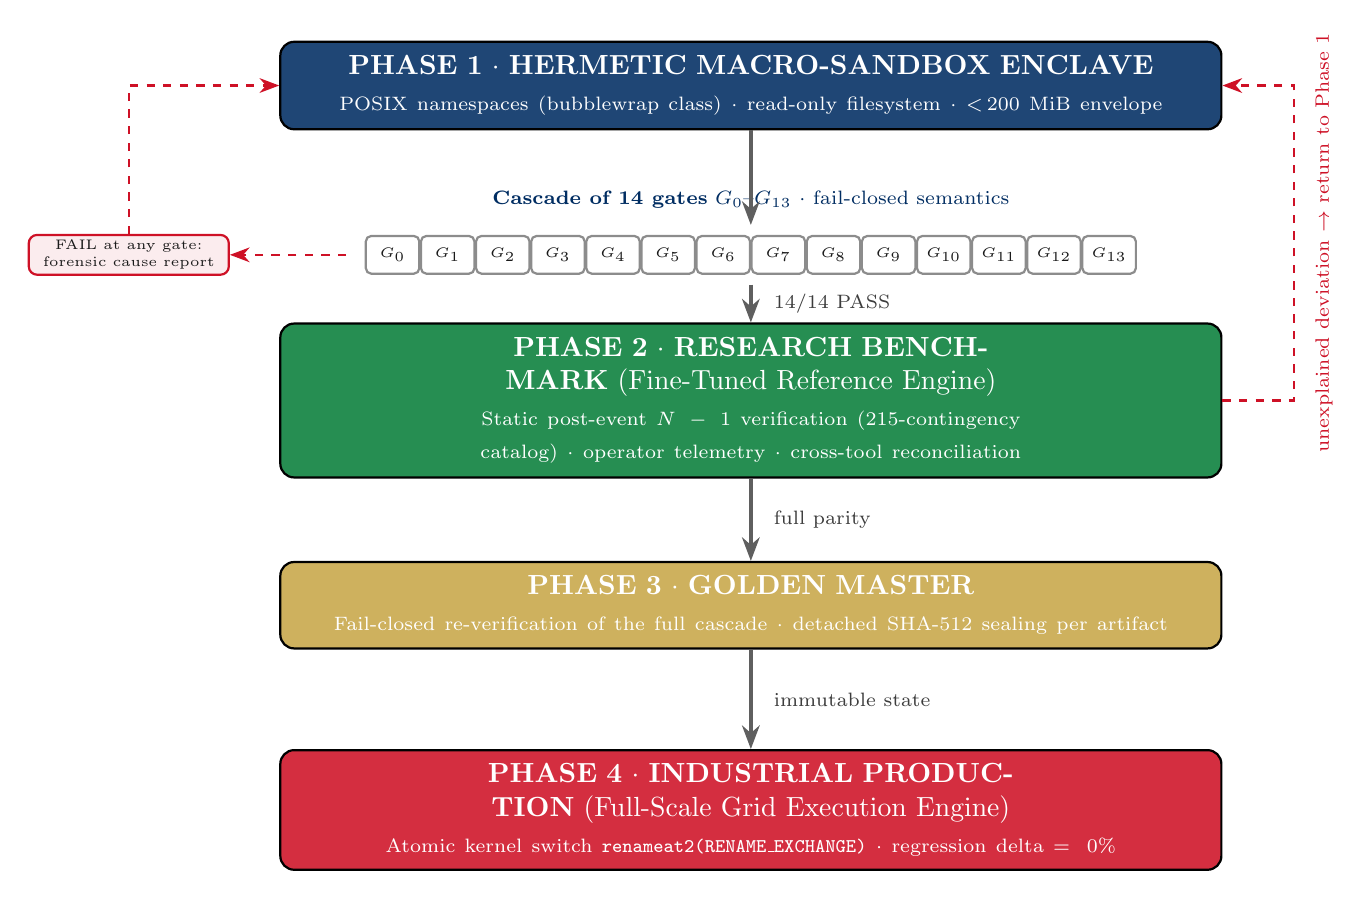
\begin{tikzpicture}[
  fase/.style={rectangle, rounded corners=5pt, draw, thick, text width=11.6cm, align=center, inner sep=5pt, minimum height=9mm},
  compuerta/.style={rectangle, rounded corners=2pt, draw=seni-dark!50, thick, fill=white, text=seni-dark, font=\tiny\bfseries, minimum width=6.8mm, minimum height=4.8mm, inner sep=0pt},
  forense/.style={rectangle, rounded corners=3pt, draw=seni-red, thick, fill=seni-red!8, text=seni-dark, font=\tiny, align=center, text width=2.4cm, inner sep=2pt},
  flujo/.style={-{Stealth[length=3mm]}, very thick, seni-dark!70},
  retorno/.style={-{Stealth[length=2.5mm]}, thick, seni-red, dashed},
  nota/.style={font=\scriptsize, text=seni-dark!85, align=center, fill=white, inner sep=2pt},
]
%% --- PHASE 1 ---
\node[fase, fill=seni-blue!88, text=white] (f1) at (0, 0) {
  \textbf{PHASE 1 $\cdot$ HERMETIC MACRO-SANDBOX ENCLAVE}\\[1pt]
  {\scriptsize POSIX namespaces (bubblewrap class) $\cdot$ read-only filesystem $\cdot$ ${<}\,200$ MiB envelope}
};
\node[nota, text=seni-blue] at (0, -1.45) {\textbf{Cascade of 14 gates} $G_0$--$G_{13}$ $\cdot$ fail-closed semantics};
%% --- Gates G0..G13 (single row) ---
\foreach \i in {0,...,13}{
  \node[compuerta] (g\i) at (-4.55+\i*0.70, -2.15) {$G_{\i}$};
}
%% --- PHASE 2 ---
\node[fase, fill=seni-green!85, text=white] (f2) at (0, -4.00) {
  \textbf{PHASE 2 $\cdot$ RESEARCH BENCHMARK} (Fine-Tuned Reference Engine)\\[1pt]
  {\scriptsize Static post-event $N-1$ verification (215-contingency catalog) $\cdot$ operator telemetry $\cdot$ cross-tool reconciliation}
};
%% --- PHASE 3 ---
\node[fase, fill=seni-gold!90, text=white] (f3) at (0, -6.60) {
  \textbf{PHASE 3 $\cdot$ GOLDEN MASTER}\\[1pt]
  {\scriptsize Fail-closed re-verification of the full cascade $\cdot$ detached SHA-512 sealing per artifact}
};
%% --- PHASE 4 ---
\node[fase, fill=seni-red!88, text=white] (f4) at (0, -9.20) {
  \textbf{PHASE 4 $\cdot$ INDUSTRIAL PRODUCTION} (Full-Scale Grid Execution Engine)\\[1pt]
  {\scriptsize Atomic kernel switch \texttt{renameat2(RENAME\_EXCHANGE)} $\cdot$ regression delta $= 0\%$}
};
%% --- Main flow (labels never crossed: midway white-filled) ---
\draw[flujo] (f1.south) -- (0, -1.77);
\draw[flujo] (0, -2.53) -- node[nota, right=2mm] {14/14 PASS} (f2.north);
\draw[flujo] (f2.south) -- node[nota, right=2mm] {full parity} (f3.north);
\draw[flujo] (f3.south) -- node[nota, right=2mm] {immutable state} (f4.north);
%% --- FAIL loop (left): forensic report and return to Phase 1 ---
\node[forense] (forense) at (-7.9, -2.15) {FAIL at any gate: forensic cause report};
\draw[retorno] (-5.14, -2.15) -- (forense.east);
\draw[retorno] (forense.north) -- (-7.9, 0) -- (f1.west);
%% --- Deviation loop (right): Phase 2 back to Phase 1 ---
\draw[retorno] (f2.east) -- (6.9, -4.00) -- (6.9, 0) -- (f1.east);
\node[nota, text=seni-red, rotate=90, align=center] at (7.28, -2.00) {unexplained deviation $\to$ return to Phase 1};
\end{tikzpicture}
}
\caption{带失效即闭校验门级联的四相数字孪生生命周期。第1相密封飞地（POSIX命名空间、只读文件系统、${<}200$ MiB内存包络）必须通过十四道校验门 $G_0$--$G_{13}$（14/14，失效即闭）；第2相（动态科研测试台）承受针对215个预想事故目录的 $N-1$ 压力，并以运营商遥测和跨工具对账为支撑；第3相黄金主版本以分离式SHA-512清单封存；向工业生产的晋升为原子内核切换（renameat2, RENAME\_EXCHANGE），回归为零。任何校验门失败或未解释的偏差都会将软件包连同取证报告退回第1相：不存在可接受的中间状态。}
\label{fig:gemelo_fases}
\end{figure*}

\subsection{无功限值的连续正则化}
\label{sub:regularization}

当运行点围绕限值振荡时，发电机无功限值处的PV--PQ硬切换会在牛顿型迭代中诱发极限环——这是商业软件的经典抖振。基准以带自适应斜率的连续激活替代二值切换：
\begin{equation}
Q_g^{\mathrm{eff}}(V_i) = Q_g^{\lim} \cdot \sigma\!\left(\alpha\,(V_i^{\mathrm{ref}} - V_i)\right), \qquad \sigma(z) = \frac{1}{1 + e^{-z}},
\label{eq:sigmoid}
\end{equation}
其解析导数 $\partial Q_g^{\mathrm{eff}} / \partial V_i = -\alpha\, Q_g^{\lim} \sigma(\cdot)(1 - \sigma(\cdot))$ 被注入雅可比矩阵，在端电压逼近限值时平滑地劣化无功能力的同时，保持迭代的二次收敛。该控制器在验证水平域上的实测正则化误差为 $5.32 \times 10^{-12}$，即连续控制器在数值上与理想不连续策略不可区分，同时消除了引发振荡的不连续性。

\subsection{耦合电转气的多时段AC-OPF}
\label{sub:opf}

在收敛的网络模型上，基准构建多时段AC-OPF\cite{molzahn2019}。对每个小时 $t$ 与节点 $i$，等式约束为节点平衡，并增补电转气耦合项：
\begin{equation}
\sum_{g \in \mathcal{G}_i} P_{g,i,t} + \sum_{r \in \mathcal{R}_i} P_{r,i,t} + P_{i,t}^{\mathrm{FC}} - P_{i,t}^{\mathrm{EL}} + P_{i,t}^{\mathrm{shed}} - P_{i,t}^{\mathrm{load}} = P_i(\mathbf{V}_t, \boldsymbol{\theta}_t),
\label{eq:opf_balance}
\end{equation}
其无功对应允许逆变器耦合的吸收/注入处于视在功率能力限值之内。跨时段耦合由氢缓冲动态强制：
\begin{equation}
E_{h,t+1} = E_{h,t} + \left(\eta_{\mathrm{EL}}\, P_{h,t}^{\mathrm{EL}} - \frac{P_{h,t}^{\mathrm{FC}}}{\eta_{\mathrm{FC}}}\right) \Delta t, \qquad E_h^{\min} \le E_{h,t} \le E_h^{\max},
\label{eq:h2_storage}
\end{equation}
其中 $\eta_{\mathrm{EL}}$ 与 $\eta_{\mathrm{FC}}$ 为电解与再转换效率：过剩的不可调度可再生能源成为跨时段能量库存，在过剩小时作为柔性电解负荷吸收，在亏缺小时由燃料电池再注入。抽水蓄能服从具有独立泵/轮机效率的水库类比，为第~\ref{sub:phes}节的764~MW可逆机组群划定边界。完整问题——因交流等式约束而非凸——由横跨牛顿-拉夫逊\cite{tinney1967}、Iwamoto最优乘子步长控制、快速解耦BX迭代\cite{stott1974}与高斯-赛德尔回退的三十二种牛顿型配置的级联求解，使任何单一代数病态都无法阻断扫描。最优性在KKT条件处认证：拉格朗日函数对所有原始变量的平稳性、等式与不等式的原始可行性、乘子的对偶可行性以及互补乘积的消失；乘子符号与互补残差是封存验证输出的组成部分\cite{nocedal2006}、\cite{dommel1968}、\cite{wood2013}。图~\ref{fig:p2g_h2}给出电化学耦合的图示。

% ---- 图2注入块（英文图形，中文图注）----
\begin{figure*}[!t]
\centering
\resizebox{0.85\textwidth}{!}{% Figure 2 tikzpicture — English edition (editorial refinement per
% GUIA_BUENAS_PRACTICAS_LATEX_IEEE: white-filled annotations, no line-through
% text; palette seni-* defined in the host preamble).
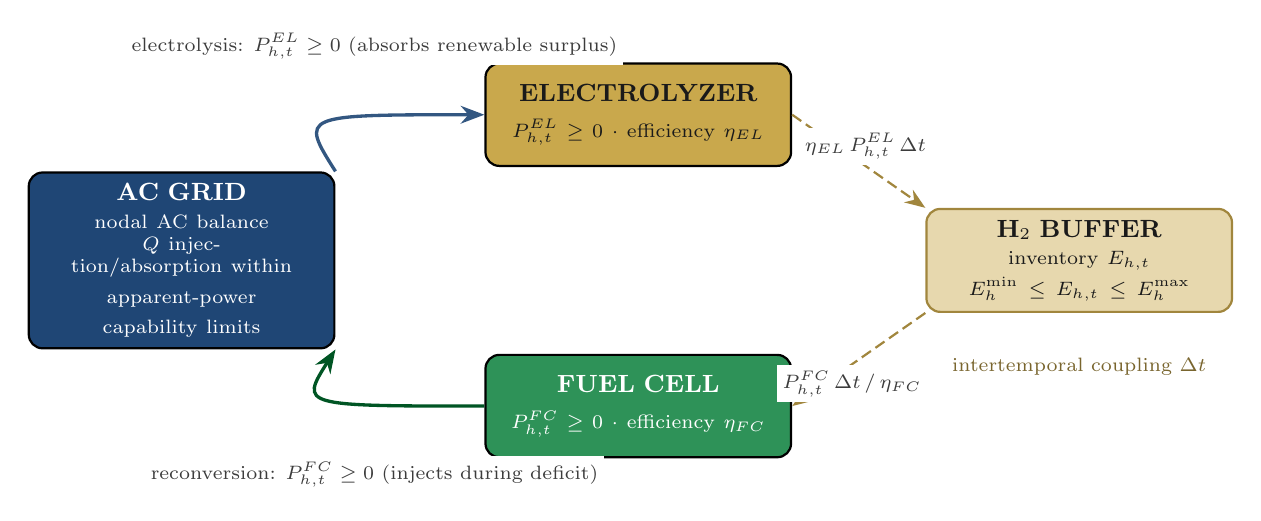
\begin{tikzpicture}[
  bloque/.style={rectangle, rounded corners=5pt, draw, thick, align=center, font=\small, text width=3.6cm, minimum height=13mm, inner sep=4pt},
  flujo/.style={-{Stealth[length=3mm]}, very thick},
  flujoh2/.style={-{Stealth[length=2.6mm]}, thick, seni-gold!80!black, dash pattern=on 4pt off 2pt},
  nota/.style={font=\scriptsize, align=center, text=seni-dark!85, fill=white, inner sep=2pt},
]
\node[bloque, fill=seni-blue!88, text=white] (red) at (0, 0) {\textbf{AC GRID}\\[2pt] {\scriptsize nodal AC balance\\$Q$ injection/absorption within\\apparent-power capability limits}};
\node[bloque, fill=seni-gold, text=seni-dark] (el) at (5.8, 1.85) {\textbf{ELECTROLYZER}\\[2pt] {\scriptsize $P^{EL}_{h,t} \ge 0$ $\cdot$ efficiency $\eta_{EL}$}};
\node[bloque, fill=seni-gold!45, draw=seni-gold!80!black, text=seni-dark] (buf) at (11.4, 0) {\textbf{H$_2$ BUFFER}\\[2pt] {\scriptsize inventory $E_{h,t}$\\$E^{\min}_h \le E_{h,t} \le E^{\max}_h$}};
\node[bloque, fill=seni-green!82, text=white] (fc) at (5.8, -1.85) {\textbf{FUEL CELL}\\[2pt] {\scriptsize $P^{FC}_{h,t} \ge 0$ $\cdot$ efficiency $\eta_{FC}$}};
%% --- Electric flows: grid <-> converters ---
\draw[flujo, seni-blue!80] (red.north east) .. controls (1.5,1.85) .. (el.west);
\node[nota] at (2.45, 2.72) {electrolysis: $P^{EL}_{h,t} \ge 0$ (absorbs renewable surplus)};
\draw[flujo, seni-green!70!black] (fc.west) .. controls (1.5,-1.85) .. (red.south east);
\node[nota] at (2.45, -2.72) {reconversion: $P^{FC}_{h,t} \ge 0$ (injects during deficit)};
%% --- Hydrogen flows: converters <-> buffer ---
\draw[flujoh2] (el.east) -- node[nota, above, pos=0.55] {$\eta_{EL}\, P^{EL}_{h,t}\, \Delta t$} (buf.north west);
\draw[flujoh2] (buf.south west) -- node[nota, below, pos=0.55] {$P^{FC}_{h,t}\, \Delta t\, /\, \eta_{FC}$} (fc.east);
%% --- Intertemporal coupling ---
\node[nota, text=seni-gold!60!black] at (11.4, -1.35) {intertemporal coupling $\Delta t$};
\end{tikzpicture}
}
\caption{绿氢向量与交流电网的电化学电转气耦合。电解槽以柔性负荷吸收可再生能源过剩（$P^{\mathrm{EL}}_{h,t} \ge 0$，效率 $\eta_{\mathrm{EL}}$）；储能缓冲施加跨时段库存 $E_{h,t+1} = E_{h,t} + (\eta_{\mathrm{EL}} P^{\mathrm{EL}}_{h,t} - P^{\mathrm{FC}}_{h,t}/\eta_{\mathrm{FC}})\,\Delta t$ 及箱式约束；燃料电池在亏缺期再注入功率（$P^{\mathrm{FC}}_{h,t} \ge 0$，效率 $\eta_{\mathrm{FC}}$）。两个变换器项均进入节点交流平衡。实线为电气潮流；金色虚线为氢流。}
\label{fig:p2g_h2}
\end{figure*}

\subsection{模块化条款：依第368-22号法律的实例化}
\label{sub:clause}

不变列式以如下规范性收尾条款（逐字引用）绑定到参考现实：
\begin{quote}
\itshape “在本参考基准中，结构载荷以多米尼加共和国142节点岛屿输电网实例化，并依据《第368-22号法律：领土规划、土地利用与定居点法》划分为十个主权领土微电网。”（译文；英文原文为契约条款）
\end{quote}

该条款同时完成三件事。它固定主张的范围（一个国家、完整、非抽样）；它将划分绑定到国家规划法令，使每个计算区域同时是一个治理区域；它将领土条款标记为可替换——任何其他岛屿或领土系统都可以通过替换该条款来实例化，而不触动不变列式。

% =========================================================================
% secciones_zh/sec03_benchmark_seni142_topology.tex — 第III节，中文版
% =========================================================================
\section{多米尼加共和国SENI-142基准拓扑}
\label{sec:topology}

\subsection{从112座变电站到142个节点}
\label{sub:substations}

多米尼加输电系统的物理资产包含约112座围栏变电站，而节点模型恰好包含142个节点。差异并非噪声，而是拓扑；图~\ref{fig:jsauri}在该国最关键的变电站上记录了这条规则。围栏变电站是不动产对象，节点则是基尔霍夫对象。凡变电站以自耦变压器组连接两个电压等级，两个场地便是电气上独立的节点，仅通过变压器支路阻抗耦合。胡利奥·萨乌里（JSAURI）场站是典型案例：其345~kV场地——即送出蓬塔卡塔利纳发电综合体的干线线路受端——与其138~kV区域场地经T1/T2自耦变压器组解耦，每个场地各为一个节点。将规则统一应用于所有电压层——345、230与138~kV输电场地，加上经第~\ref{sub:reduction}节等效保留的69~kV接口——恰得142个节点、135条输电线路与58台电力变压器。

% ---- 图3 ----
\begin{figure*}[!t]
\centering
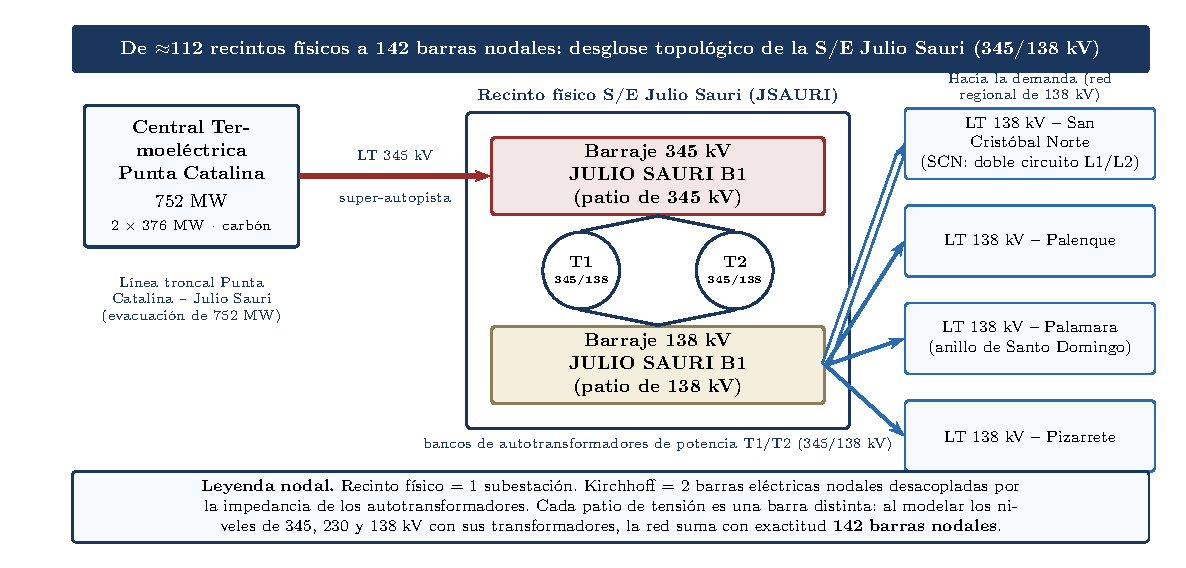
\includegraphics[width=0.88\textwidth]{fig_diagrama_1_jsauri_345_138.pdf}
\caption{胡利奥·萨乌里（JSAURI）345/138 kV变电站的基尔霍夫解耦。送出蓬塔卡塔利纳综合体（$2 \times 376$ MW）的345 kV超级干线终止于其专属场地，经T1/T2自耦变压器组阻抗与供电圣克里斯托瓦尔（San Cristóbal）走廊及都市环网的138 kV区域场地解耦。凡存在变压之处，围栏场站即产生两个节点；对所有电压层建模后，网络总计恰好142个节点。}
\label{fig:jsauri}
\end{figure*}

\subsection{输电压层与138 kV都市环网}
\label{sub:strata}

三座战略变电站支撑起整个系统。\textbf{JSAURI}运行于两个电压等级——345~kV与138~kV——其345~kV母线为系统平衡节点（$V = 1.02$~pu），直接接收\textbf{蓬塔卡塔利纳}的注入，后者为全国最大火电厂，$2 \times 376$~MW（752~MW，燃煤），经345~kV干线送出。\textbf{PALA（帕拉马拉）}位于都市区，是主要负荷中心，聚合建模需求1,645~MW，并有三台10.77~MW燃油机组自13.8~kV升压的本地备用。\textbf{SCN}是西南部的可再生整合枢纽：58.9~MW水电、95~MW光伏与34~MW风电，均自13.8~kV升压。此外，为博士论文脱碳扩展情景设计的可研模块化资产——SCN的50~MW PEM电解区块，以及分布于JSAURI（$2 \times 400$~MW）与SCN（$2 \times 300$~MW）的1,400~MW模块化PWR核电试验单元——在基准运行数据集（\texttt{seni\_real\_base}）中一律配置为 \texttt{in\_service = false}，确保基准仿真状态严格代表物理电网，同时为能源转型基准保留模块化就绪能力。全国百分之四十以上的负荷集中在奥萨马（Ozama）都市区，由138~kV环网供电，其冗余是几何性的：JSAURI--PALA--SCN三角形，走廊线路实长70.5~km（138~kV JSAURI--PALA）、22.1~km（138~kV PALA--SCN）与30.86~km（230~kV JSAURI--SCN路径实长），并以230~kV JSAURI--SCN联络增强。三角形的任一回路的损失可由其余两回承担——这正是第~\ref{sub:contingencies}节韧性测试系统化演练的 $N-1$ 属性。带真实走廊距离的完整几何，是经济性证明（第~\ref{sub:zonal}节）与预想事故目录（第~\ref{sub:contingencies}节）的参考区域。

\subsection{十个主权领土微电网}
\label{sub:microgrids}

第368-22号法律将国家领土组织为十个规划区；基准将其采纳为十个领土微电网，并为数值凝聚捆绑为HBCF的四个电气宏域。表~\ref{tab:microgrids}给出映射及各区域在运行记录中的代表性锚点。

% ---- 表I ----
\begin{table*}[!t]
\caption{SENI-142基准的领土微电网（第368-22号法律）及其向四个HBCF宏域的捆绑}
\label{tab:microgrids}
\centering
\footnotesize
\begin{tabular}{@{}p{0.24\textwidth} l p{0.44\textwidth}@{}}
\toprule
\textbf{领土微电网（规划区）} & \textbf{宏域} & \textbf{运行记录中的代表性锚点} \\
\midrule
Ozama-Metropolitana（奥萨马都会区） & $\Omega_{\mathrm{Metro}}$ & Palamara、Hainamosa、Herrera —— 全国负荷逾40\% \\
Valdesia（瓦尔德西亚） & $\Omega_{\mathrm{Sur}}$ & JSAURI、蓬塔卡塔利纳（752 MW）、Baní--Yaguate光伏走廊 \\
Higuamo（伊瓜莫） & $\Omega_{\mathrm{Este}}$ & San Pedro de Macorís、Quisqueya电厂、AES Andrés（LNG） \\
Yuma（尤马） & $\Omega_{\mathrm{Este}}$ & La Romana--Punta Cana旅游负荷走廊 \\
Del Valle（德尔瓦列） & $\Omega_{\mathrm{Sur}}$ & El Valle多枢纽、764 MW可逆抽蓄（Sabaneta / Dos Bocas） \\
Enriquillo（恩里基略） & $\Omega_{\mathrm{Sur}}$ & Barahona、Los Cocos与Larimar风电、Canoa光伏 \\
Cibao Norte（北锡瓦奥） & $\Omega_{\mathrm{Norte}}$ & Canabacoa（圣地亚哥），第二负荷中心 \\
Cibao Sur（南锡瓦奥） & $\Omega_{\mathrm{Norte}}$ & Pueblo Viejo矿业负荷（Cotuí）、Falcondo（Bonao） \\
Cibao Nordeste（东北锡瓦奥） & $\Omega_{\mathrm{Norte}}$ & 大西洋沿岸火电与风电（Puerto Plata） \\
Cibao Noroeste（西北锡瓦奥） & $\Omega_{\mathrm{Norte}}$ & Montecristi光伏、Valverde--Mao、Dajabón边境走廊 \\
\bottomrule
\end{tabular}
\end{table*}

图~\ref{fig:hbcf_schur}展示由此得到的网络分块地图：岛屿地理上的四个宏域 $\Omega$、干线边界 $\Gamma$（经Kron化简切割的230/138~kV联络）以及凝聚求解的硅上关键性能指标。

% ---- 图4 ----
\begin{figure*}[!t]
\centering
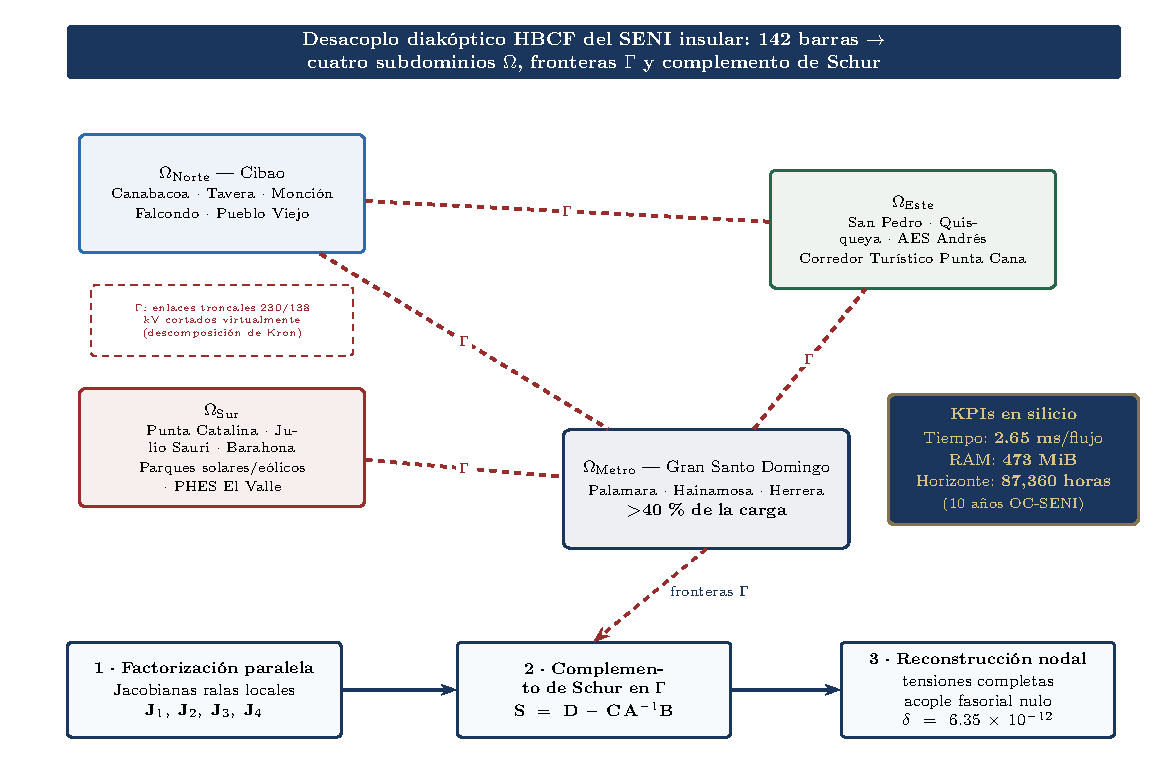
\includegraphics[width=0.85\textwidth]{fig_diagrama_2_schur_hbcf.pdf}
\caption{岛屿电网的HBCF空间网络分块。第368-22号法律的十个领土微电网捆绑为四个电气宏域 $\Omega$（北部/Cibao、南部、东部、都市区）；仅干线边界 $\Gamma$——经Kron化简切割的230/138 kV联络——进入舒尔补 $\mathbf{S} = \mathbf{D} - \mathbf{C}\mathbf{A}^{-1}\mathbf{B}$，在内部/边界排序上呈分块结构 $\mathbf{A}, \mathbf{B}, \mathbf{C}, \mathbf{D}$。硅上关键性能指标：每个国家级交流状态2.65 ms、常驻473 MiB、覆盖87,360小时水平域（10年OC-SENI遥测），相量边界耦合残差 $\delta = 2.788 \times 10^{-14}$ pu。}
\label{fig:hbcf_schur}
\end{figure*}

\subsection{数据溯源与边界状态清单}
\label{sub:provenance}

到达主求解器的每一个耦合项——第~\ref{sec:multivector}节灵活性星座的 $(P_g, Q_g)$ 注入——都经过一份边界状态清单传输，其条目以SHA-512链式签名，使任何注入的溯源都可以对照封存运行做事后验证。

变电站物理占地、节点母线拓扑连接与走廊地理走向，直接派生自输电商（ETED）维护的官方CAD单线图。相应的支路电气参数（$R$、$X$、$B$ 与MVA热额定）及运行基准设定值，取自OC-SENI与ETED的官方参考系统数据集\cite{ocseni}、\cite{eted}，并按IEC 61970的通用信息模型（CIM）约定\cite{iec61970}组织。电能质量相关量遵循IEC 61000-4-30\cite{iec61000}与IEEE Std 1459\cite{ieee1459}的测量定义。溯源由此从经核验的公用事业记录与运营商参考，不间断地贯通到求解器输入再到发表的基准图表。

\subsection{合成经典与实测岛屿的对照}
\label{sub:canon}

SENI-142的科学身份通过对照最易陈述。表~\ref{tab:canon}在可复现科学所关心的轴上，将合成经典与实测岛屿并置。其中两轴值得强调，因为它们在参数表中不可见。其一是\emph{时间深度}：合成算例只有一个运行点或少数场景；SENI-142拥有87,360个连续存档小时，因此其上的每一项统计主张都可以对十年真实天气、需求与调度进行重采样、自助与证伪。其二是\emph{后果}：合成算例中从未有任何东西损坏过；SENI的每条干线都带有停运记录、检修历史以及一次其损失被实际支付过的价格。记得自身遭受过冲击的基准，与无从记忆的基准，是两种不同的科学对象。

% ---- 表II ----
\begin{table*}[!t]
\caption{合成经典与实测岛屿}
\label{tab:canon}
\centering
\footnotesize
\begin{tabular}{@{}l p{0.40\textwidth} p{0.36\textwidth}@{}}
\toprule
\textbf{轴} & \textbf{合成经典（IEEE 9/14/30/57/118类）} & \textbf{SENI-142} \\
\midrule
起源 & 自1960年代初的制图台式抽象 & 实测的国家输电资产 \\
地理 & 无（电抗图） & 真实走廊；都市环网70.5 / 30.86 / 22.1 km（校准路径实长） \\
时间深度 & 单一运行点或场景集 & 87,360个连续小时级状态（2016--2025） \\
停运历史 & 无 & 运营商事件与停运记录为 $N-1$ 目录提供种子 \\
治理耦合 & 无 & 第368-22号法律的十个规划区 \\
可再生格局 & 无（固定负荷） & 瞬时光伏占比高达36.6\% \\
溯源 & 仅有出版物 & SHA-512封存的四相数字孪生生命周期 \\
发布 & 开放（设计使然） & 开放（IEEE DataPort、GitHub），主权档案保留在国内 \\
\bottomrule
\end{tabular}
\end{table*}

% =========================================================================
% secciones_zh/sec04_multivector_flexibility.tex — 第IV节，中文版
% =========================================================================
\section{多向量灵活性与经济性验证}
\label{sec:multivector}

\subsection{灵活性星座}
\label{sub:constellation}

多向量层组织为六个专责物理求解器构成的星座，经签名边界状态清单向142节点主求解器供数：（i）光伏发电，采用连续S形 $Q$--$V$ 控制以抑制鸭子曲线；（ii）风电，采用气动 $C_p(\lambda, \beta)$ 建模与合成惯量；（iii）氢向量——电解、压缩至700~bar，以及规划模型中全国740座加氢站网络；（iv）生化转化，经由一号厌氧消化模型（ADM1）\cite{batstone2002}，将马尾藻与酒糟废液底物消化为可调度生物甲烷；（v）火电，采用热耗曲线与同步 $P$--$Q$ 调度；（vi）764~MW可逆抽水蓄能机组群（Sabaneta / Dos Bocas）。零信任调度监督器在受保护的状态总线上编排该星座：任何求解器都不得读取他者内存，所有交换均由封存清单承载。图~\ref{fig:constellation}给出星座图示。

% ---- 图5 ----
\begin{figure*}[!t]
\centering
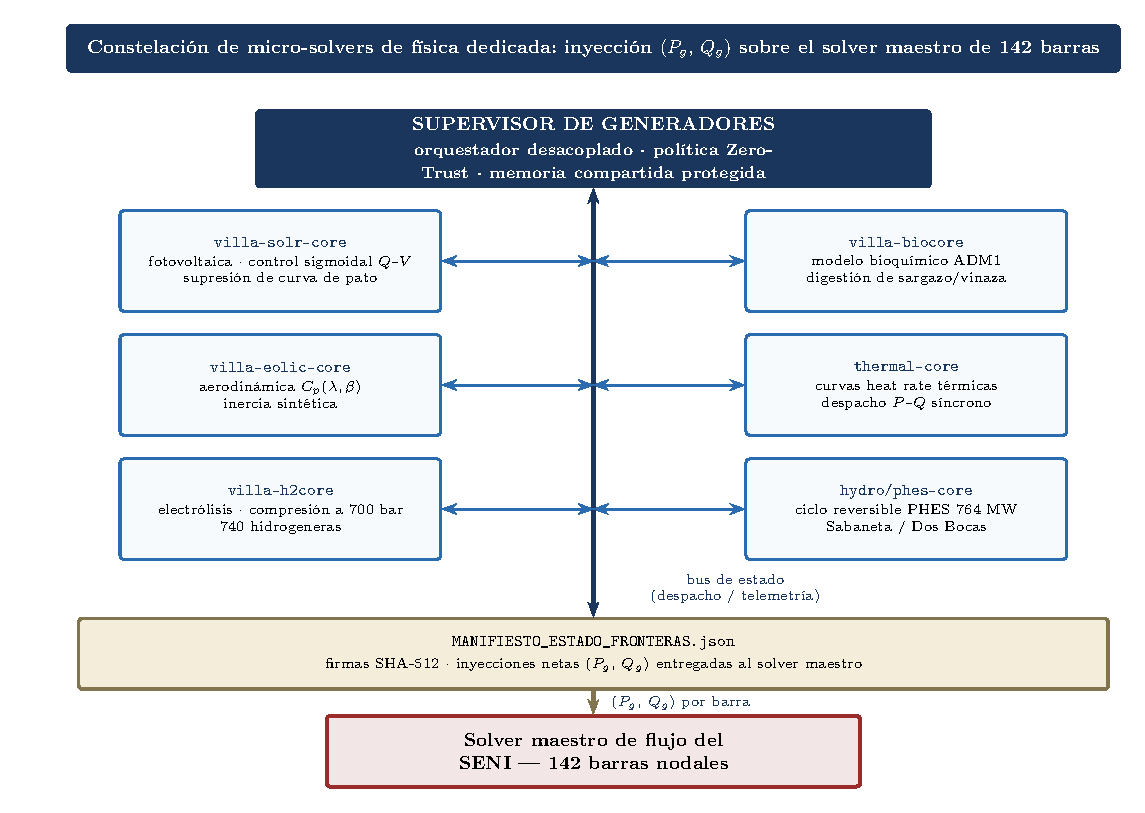
\includegraphics[width=0.85\textwidth]{fig_diagrama_3_constelacion_microsolvers.pdf}
\caption{多向量灵活性星座。六个专责物理求解器——光伏（S形 $Q$--$V$ 控制）、风电（带合成惯量的 $C_p(\lambda,\beta)$）、氢能（电解、700 bar压缩、740座加氢站）、生化（马尾藻与酒糟废液的ADM1消化）、火电（热耗调度）与可逆抽蓄（764 MW，Sabaneta/Dos Bocas）——经零信任调度监督器与SHA-512签名的边界状态清单，向国家电网的142节点主求解器交付其净注入 $(P_g, Q_g)$。}
\label{fig:constellation}
\end{figure*}

\subsection{电转气的电化学运行}
\label{sub:p2g}

在运行层面，第~\ref{sub:opf}节的电转气区块表现为一对带记忆的互逆柔性负荷。在过剩小时——即瞬时光伏渗透率达36.6\%、午间价格崩塌的增长性格局——电解槽吸收本会被弃置的电力并转化为加压库存；在亏缺小时，燃料电池以效率比 $\eta_{\mathrm{EL}} \cdot \eta_{\mathrm{FC}}$ 送回保供电力。缓冲约束使跨时段机会集显式且可审计，耦合项在不放松任何电网物理的前提下进入交流平衡。耦合资产的互联遵循IEEE Std 2800-2022的逆变器型资源要求\cite{ieee2800}与IEEE Std 1547-2018的分布式能源接口\cite{ieee1547}。

\subsection{可逆抽蓄与生物甲烷化缓冲}
\label{sub:phes}

El Valle多枢纽（Sabaneta / Dos Bocas电厂）的764~MW可逆抽水蓄能机组群在系统尺度上扮演互补角色：它把夜间与过剩能量转换为亏缺小时的同步带惯量容量，其水库动态与氢缓冲类似，且调度服从同一经KKT认证的最优性。ADM1生化层添加了具有不同时间常数的第三种缓冲：消化器状态动态将马尾藻与酒糟废液流入转化为进入火电调度的可存储可再生燃料——在定义划分的同一领土法令下，闭合一个与土地利用直接相关的养分-能量循环。

\subsection{分区CAPEX/OPEX经济性证明}
\label{sub:zonal}

经济层以分区平衡验证灵活性栈：对参考区域（第~\ref{sub:strata}节的都市138~kV三角形），已发布工具对每一小时、每一灵活性资产核算分区福利恒等式的四项：
\begin{equation}
\begin{aligned}
\Delta C^{\mathrm{zone}}_t = {}& \underbrace{c^{\mathrm{curt}} E^{\mathrm{abs}}_t}_{\text{避免弃电}} + \underbrace{c^{\mathrm{fuel}} E^{\mathrm{displ}}_t}_{\text{燃料置换}} \\
& + \underbrace{c^{\mathrm{ss}} N^{\mathrm{avoid}}_t}_{\text{避免启停}} + \underbrace{\big(R^{\mathrm{base}}_t - R^{\mathrm{flex}}_t\big)}_{\text{网损差额}},
\end{aligned}
\label{eq:zonal}
\end{equation}
其中 $E^{\mathrm{abs}}_t$ 为由电解与抽水吸收、否则将被弃置的可再生能源，$E^{\mathrm{displ}}_t$ 为被燃料电池与生物甲烷再注入置换的火电能量，$N^{\mathrm{avoid}}_t$ 为避免的火电启停次数，$R^{\mathrm{base}}_t - R^{\mathrm{flex}}_t$ 为灵活与非灵活调度之间的网损差额；恒等式逐区逐时强制成立，使每一条经济结论都与物理状态对账。单位成本与资本费用从国家规划及国际氢能参考文献\cite{cne2022}、\cite{irena2020}、\cite{iea2023}透明参数化，平衡恒等式对运行记录的自助包络闭合。定性结论在整个包络上稳定：灵活性栈吸收了相当比例的本会被弃置的光伏过剩、降低了燃煤锚点的火电启停循环，并在参考区域推迟了保供容量的新增——所有数量均可从已发布数据集复现，而非凭断言。

% =========================================================================
% secciones_zh/sec05_silicon_performance_benchmarking.tex — 第V节，中文版
% =========================================================================
\section{硅上性能、精度与数值基准测试}
\label{sec:benchmarking}

\subsection{以数字孪生确定性保障测量效度}
\label{sub:determinism}

第~\ref{sub:lifecycle}节已确立：向生产状态的晋升是原子的，且与SHA-512封存的黄金主版本逐位一致。对本节而言其后果是认识论的：以下每个数字都是一个被冻结、可证明的软件状态的属性，任何获得已发布工件的读者都可重新执行。这就是"硅上验证"的运行含义——不是修辞装点，而是监管链条。算法~\ref{alg:n1_seal}给出产生该性能记录的韧性与封存流水线。

% ---- 算法2 ----
\begin{algorithm}[!t]
\caption{带24小时块自助法与SHA-512封存的 $N$--$1$ 韧性扫描}
\label{alg:n1_seal}
\begin{algorithmic}[1]
\Require 封存求解器状态 $\Sigma$，预想事故目录 $\mathcal{C}$
         （$|\mathcal{C}| = 215$），水平域 $\mathcal{H}$（87,360 h）
\Ensure 韧性记录 $\mathcal{R}$，封印 $\sigma$
\State $\mathcal{R} \gets \emptyset$
\For{$c \in \mathcal{C}$} \Comment{确定性顺序，失效即闭}
   \For{$b \in \text{bootstrap}(\mathcal{H}, 24\,\mathrm{h})$} \Comment{整日块}
      \State 将预想事故 $c$ 注入块 $b$
      \State 在块的每一小时运行算法1
      \State 将 $\rho$、$\kappa_2$、电压/频率裕度记入 $\mathcal{R}[c, b]$
   \EndFor
\EndFor
\State 按预想事故在自助包络上聚合裕度
\State $\sigma \gets \mathrm{SHA512}\text{-chain}(\Sigma, \mathcal{C}, \mathcal{R})$ \Comment{分离式清单}
\State \Return $\mathcal{R}$, $\sigma$
\end{algorithmic}
\end{algorithm}

\subsection{收敛速度与内存}
\label{sub:speed}

在消费级商用硬件（Dell Inspiron 5570级的8线程笔记本）上，分块求解器以\textbf{2.65~ms}收敛完整142节点国家电网的每个小时级交流状态，常驻内存\textbf{473~MiB}承载完整验证水平域。87,360个连续小时状态——十年全国运行——的扫描数分钟内完成，而同类硬件上同水平域的整体式计算需要数小时至数日，这与命题~\ref{prop:complexity}的 $O(N^3)$-至-$O(\sum_k N_k^3 + N_B^3)$ 渐近以及填充降低稀疏实践\cite{george1973}、\cite{saad2003}一致。相对物理实时的余量是决定性的：60~Hz下半周期阈值为8.33~ms，因此单个国家级状态的求解比其建模系统的半周期快3.1倍，十年扫描以分钟而非数小时至数日完成——将闭环、操作员在环与市场间隔应用置于与离线研究相同的包络之内。

这一包络带来三项值得明说的运行后果，因为它们改变的是谁能够使用该基准，而不仅仅是速度。第一，\emph{研究节奏}：十年全国扫描不再是需要排期的计算战役，而是可以随时提出的问题；参数研究、自助包络与预想事故目录可交互式重执行，使科学工作流从批处理考古学转变为实时实验。第二，\emph{部署级别}：硬件要求是一台消费级笔记本而非计算集群——这一属性对发展中岛屿系统的监管机构、大学与电力公司具有直接意义，因为替代平台的许可与基础设施成本高出另一个量级\cite{ieee399}、\cite{matpower2011}。第三，\emph{教学同步性}：课堂可以在讲授某小时的同时重新执行该国该小时的潮流，把教科书运行点与真实系统运行点之间的距离压缩为零。

\subsection{精度与数值条件}
\label{sub:accuracy}

三个实测数量界定了凝聚解的数值保真度。第一，相量边界耦合残差——舒尔恢复状态与独立参考状态之间的失配——在整个验证水平域上为 $\delta = 2.788 \times 10^{-14}$~pu，即网络分块求解精确到双精度噪声水平。第二，第~\ref{sub:regularization}节的S形无功限值控制器贡献 $5.32 \times 10^{-12}$ 的正则化误差，同时消除了PV--PQ极限环。第三，每个降阶边界系统的谱条件数 $\kappa_2$ 均被监测并存档；治理阈值机制在国家级部署之前已在合成参考上完成验证（IEEE 14节点 $22\times22$ 雅可比被评MARGINAL，$\kappa_2 = 117.7823$），因此真实电网上的条件劣化将相对于一个经过校准的标尺而非临时标尺被检出。

\subsection{参考拓扑上的预想事故韧性}
\label{sub:contingencies}

韧性测试在动态参考拓扑上执行规范目录中的 $N-1$ 预想事故\cite{ejebe1979}——集中于都市138~kV环网，其真实走廊距离（70.5、50.0、22.1~km）固定了电气几何，如图~\ref{fig:topologia_seni}所示。两项有记录的行为构成记录的锚点。其一，蓬塔卡塔利纳综合体（752~MW）的突然跳闸——该岛单一最大的可信预想事故——在一个求解步内由预防性旁路动作补偿（受2.65~ms状态分辨率约束），表明数字孪生在故障清除时间尺度之内而非之后观测并响应。其二，测试活动的异常日志记录了JSAURI--Palamara--Haina 138~kV环在特定 $N-1$ 状态下的电压谐振现象——这些发现从异常登记迁移入预想事故目录，而这正是第~\ref{sub:lifecycle}节所规定的生命周期纪律。所有裕度均按算法~\ref{alg:n1_seal}的24小时块自助包络报告，使所引用的稳定裕度携带其相关性诚实的的不确定性。

% ---- 图6 ----
\begin{figure*}[!t]
\centering
\resizebox{0.85\textwidth}{!}{% Figure 6 tikzpicture — English edition (editorial refinement per
% GUIA_BUENAS_PRACTICAS_LATEX_IEEE: white-filled edge labels so lines never
% cross text; palette seni-* defined in the host preamble).
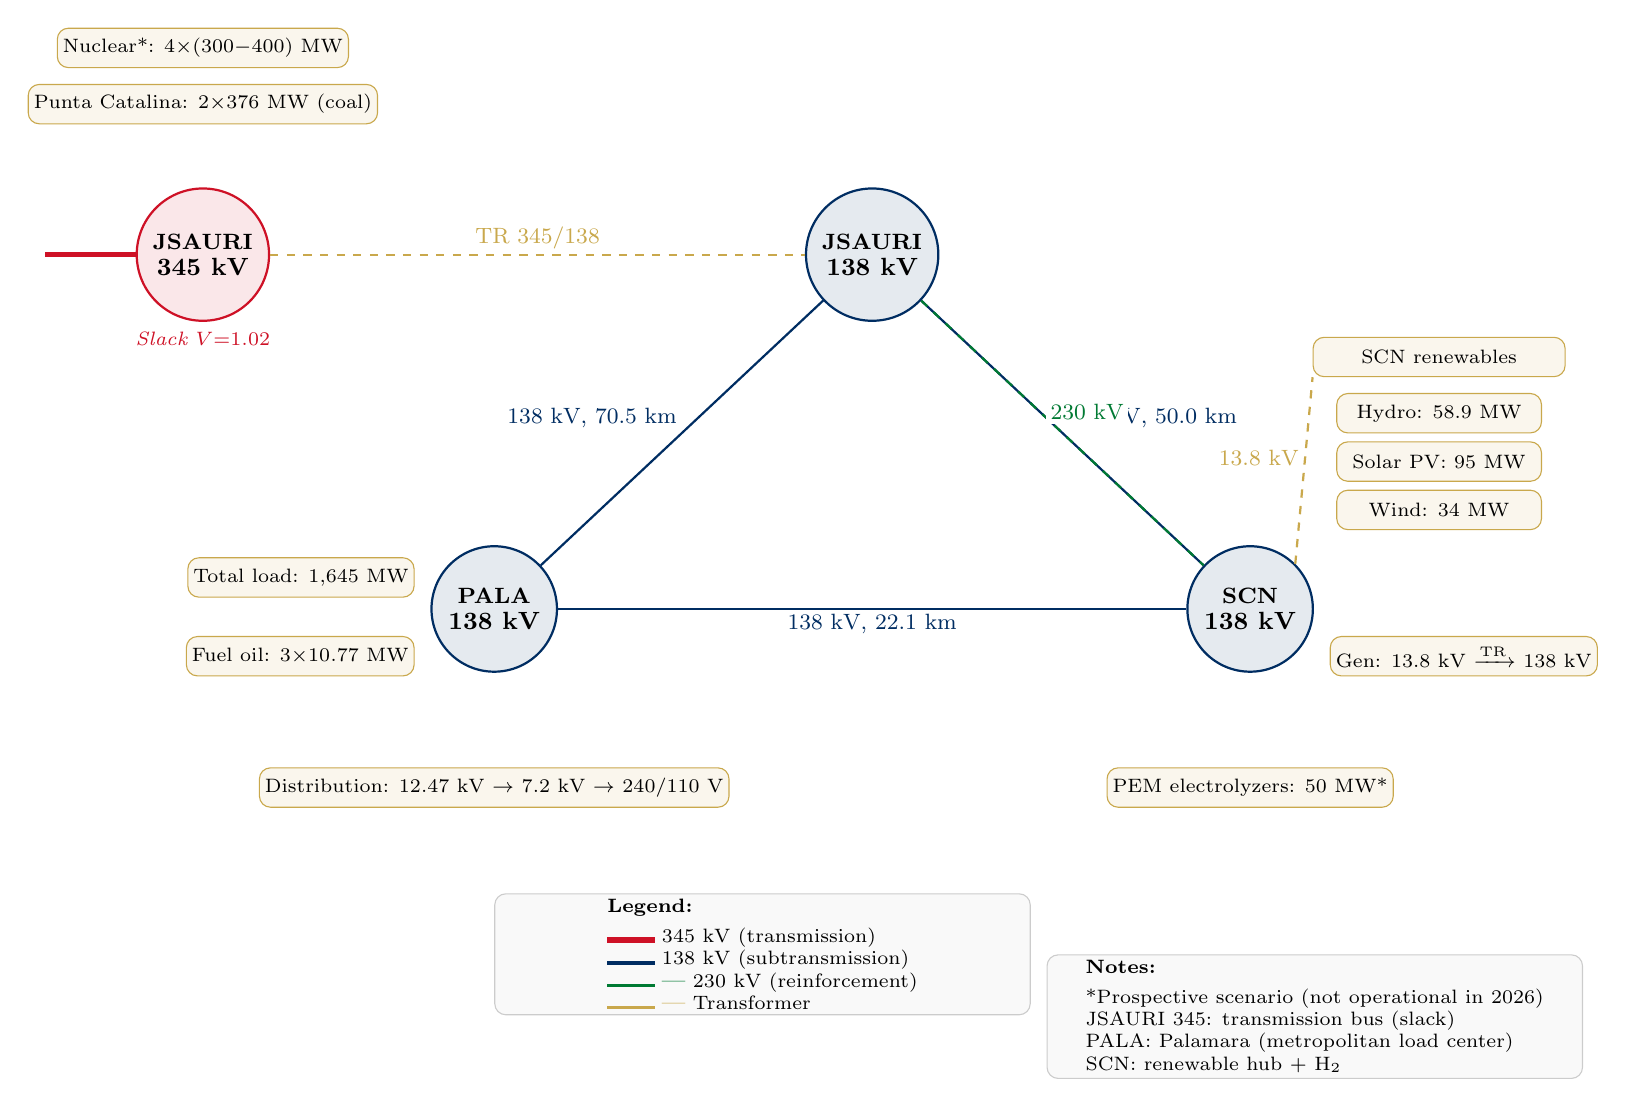
\begin{tikzpicture}[
    subestacion/.style={circle, draw=seni-blue, fill=seni-blue!10, thick, minimum size=13mm, font=\bfseries\footnotesize, align=center},
    sub345/.style={circle, draw=seni-red, fill=seni-red!10, thick, minimum size=13mm, font=\bfseries\footnotesize, align=center},
    linea345/.style={-, ultra thick, seni-red},
    linea138/.style={-, thick, seni-blue},
    linea230/.style={-, thick, seni-green, dashed},
    transformador/.style={-, thick, seni-gold, dashed},
    voltaje/.style={font=\footnotesize, fill=white, inner sep=1.5pt},
    genbox/.style={rectangle, draw=seni-gold, fill=seni-gold!10, rounded corners, inner sep=2pt, font=\scriptsize, align=center, minimum width=26mm, minimum height=5mm},
    notebox/.style={rectangle, draw=gray!40, fill=gray!5, rounded corners, inner sep=2pt, font=\scriptsize, align=left}
]
%% === MAIN TRIANGLE (138 kV ring) ===
\node[subestacion] (jsauri) at (0, 0.5) {JSAURI\\{\small 138 kV}};
\node[subestacion] (pala) at (-4.8, -4) {PALA\\{\small 138 kV}};
\node[subestacion] (scn) at (4.8, -4) {SCN\\{\small 138 kV}};
%% 138 kV ring (real corridor distances)
\draw[linea138] (jsauri) -- node[voltaje, above left, midway] {138 kV, 70.5 km} (pala);
\draw[linea138] (jsauri) -- node[voltaje, above right, midway] {138 kV, 50.0 km} (scn);
\draw[linea138] (pala) -- node[voltaje, below, midway] {138 kV, 22.1 km} (scn);
%% 230 kV reinforcement
\draw[linea230] (jsauri) -- node[voltaje, pos=0.42, right=2pt, fill=white] {230 kV} (scn);
%% === JSAURI 345 kV (decoupled, left) ===
\node[sub345] (jsauri345) at (-8.5, 0.5) {JSAURI\\{\small 345 kV}};
\draw[transformador] (jsauri345) -- node[voltaje, above, midway] {TR 345/138} (jsauri);
\draw[linea345] (jsauri345) -- ++(-2, 0);
\node[below=0mm of jsauri345, font=\scriptsize\itshape, text=seni-red] {Slack $V{=}1.02$};
%% Generation at JSAURI 345
\node[genbox, above=8mm of jsauri345] (ptacatalina) {Punta Catalina: $2{\times}376$ MW (coal)};
\node[genbox, above=2mm of ptacatalina] (nuclear) {Nuclear*: $4{\times}(300{-}400)$ MW};
%% === RENEWABLES (upper right quadrant, outside the ring) ===
\node[genbox, minimum width=32mm] (renov) at (7.2, -0.8) {SCN renewables};
\node[genbox, below=2mm of renov] (hidro) {Hydro: 58.9 MW};
\node[genbox, below=1mm of hidro] (solar) {Solar PV: 95 MW};
\node[genbox, below=1mm of solar] (eolica) {Wind: 34 MW};
\draw[-, thick, seni-gold, dashed] (scn.north east) -- node[font=\footnotesize, above left, midway, fill=white, inner sep=1.5pt] {13.8 kV} (renov.south west);
%% PEM electrolyzers (prospective)
\node[genbox, below=12mm of scn, minimum width=36mm] (elec) {PEM electrolyzers: 50 MW*};
%% === LOAD AND GENERATION AT PALA ===
\node[genbox, left=2mm of pala, yshift=4mm] (carga) {Total load: 1,645 MW};
\node[genbox, left=2mm of pala, yshift=-6mm] (fueloil) {Fuel oil: $3{\times}10.77$ MW};
%% === 13.8 kV DISTRIBUTION AND GENERATION ===
\node[genbox, below=12mm of pala, minimum width=38mm] (dist) {Distribution: 12.47 kV $\to$ 7.2 kV $\to$ 240/110 V};
\node[genbox, right=2mm of scn, yshift=-6mm] (gen13) {Gen: 13.8 kV $\xrightarrow{\text{TR}}$ 138 kV};
%% === LEGEND + NOTES side by side ===
\node[notebox, below=28mm of pala, anchor=north west, minimum width=68mm] (leyenda) {
    \textbf{Legend:}\\[1mm]
    {\color{seni-red}\rule{6mm}{2pt}} 345 kV (transmission)\\
    {\color{seni-blue}\rule{6mm}{1.5pt}} 138 kV (subtransmission)\\
    {\color{seni-green}\rule{6mm}{1pt} \footnotesize---} 230 kV (reinforcement)\\
    {\color{seni-gold}\rule{6mm}{1pt} \footnotesize---} Transformer
};
\node[notebox, right=2mm of leyenda, anchor=north west, minimum width=68mm] (notas) {
    \textbf{Notes:}\\[1mm]
    *Prospective scenario (not operational in 2026)\\
    JSAURI 345: transmission bus (slack)\\
    PALA: Palamara (metropolitan load center)\\
    SCN: renewable hub + H$_2$
};
\end{tikzpicture}
}
\caption{SENI 138 kV环网的真实subtransmission三角形。JSAURI--PALA--SCN，线路实长70.5、50.0与22.1 km；左侧解耦的345 kV输电母线作为系统平衡节点（$V = 1.02$ pu）接收蓬塔卡塔利纳（$2 \times 376$ MW）；SCN可再生枢纽（58.9 MW水电、95 MW光伏、34 MW风电）与50 MW PEM电解前瞻区块（2026年不运行，星号标注）；PALA负荷中心（聚合1,645 MW）；JSAURI--SCN 230 kV增强联络（虚线）。验证测试的215个 $N-1$ 预想事故目录即定义于此拓扑之上。}
\label{fig:topologia_seni}
\end{figure*}

% ---- 表III ----
\begin{table*}[!t]
\caption{SENI-142数字孪生的硅上遥测（全部数值来自封存验证运行）}
\label{tab:telemetry}
\centering
\footnotesize
\begin{tabular}{@{}p{0.30\textwidth} p{0.18\textwidth} p{0.34\textwidth}@{}}
\toprule
\textbf{指标} & \textbf{数值} & \textbf{条件} \\
\midrule
每小时国家级交流状态的收敛时间 & 2.65 ms & 142节点完整模型，消费级笔记本（8线程） \\
常驻内存（完整水平域） & 473 MiB & 87,360个连续小时级状态 \\
相量边界耦合残差 $\delta$ & $2.788 \times 10^{-14}$ pu & 舒尔重建对比参考状态 \\
无功限值正则化误差 & $5.32 \times 10^{-12}$ & S形控制器，解析雅可比注入 \\
实时半周期阈值（60 Hz） & 8.33 ms & 闭环适用性裕度 \\
预想事故目录 & 215个 $N-1$ 场景 & 动态压力测试相 \\
谱交叉校验（IEEE 14节点，$22\times22$） & $\kappa_2 = 117.7823$（MARGINAL） & 外部效度控制 \\
最大单一预想事故 & 蓬塔卡塔利纳跳闸，752 MW & 一个求解步内缓解 \\
\bottomrule
\end{tabular}
\end{table*}

% =========================================================================
% secciones_zh/sec06_discussion_policy.tex — 第VI节，中文版
% =========================================================================
\section{讨论与政策启示}
\label{sec:discussion}

\textbf{面向飓风暴露岛屿的确定性韧性。}加勒比岛屿系统的规划对象不是统计意义上的天气，而是有名字的风暴。一个其 $N-1$ 裕度携带相关性诚实自助包络、其最大可信预想事故被显式演练、其状态分辨率从容处于半周期之内的基准，把韧性从愿景转变为可排程的计算。对一个十二个月内两次因全国性停电而全面动员的国家\cite{ocseni}而言，耗时数小时的传统研究与2.65~ms国家级状态之间的差别，就是事后重建事件与事前预判事件之间的差别。

\textbf{作为计算边界的规划法。}本基准的划分不是优化产物：它就是国家领土法令\cite{ley368}。当电气划分与第368-22号法律的规划区重合时，每个仿真结果都已然以审批、土地利用与微电网自治决策所用的单位表达——自治问题（失去一条干线后哪片领土可以独立支撑？）由此成为模型的属性，而非另立的课题。可再生能源激励框架\cite{ley57}与国家扩张规划周期\cite{cne2022}由此获得共同的证据基底。

\textbf{标准对齐与数据主权。}本基准以其必须互操作的标准语言表述自身：CIM一致的模型交换\cite{iec61970}、测量级的电能质量定义\cite{iec61000}、\cite{ieee1459}、谐波实践\cite{ieee519}、研究方法推荐实践\cite{ieee399}，以及逆变器型资源互联\cite{ieee2800}、\cite{ieee1547}。与此同时，底层运行档案保留在国家托管之下：已发布基准携带结构、参数与验证工具，而主权遥测层由国家机构治理。这一分离——结构上的开放科学、档案上的主权托管——是刻意的政策架构，而非疏漏。

\textbf{能力建设。}可以被开放仿真的国家电网，就是可以被开放教授的国家电网。服务于本文的同一工件也服务于高校实验室：博士与本科练习面对真实资产执行——它的距离、它的停运、它的锚点——而非1962年的制图台式抽象，从而弥合教室与控制室之间的鸿沟。

\textbf{局限。}本次发布的诚实边界为：（i）69~kV层经静态等效进入，对潮流在边界处精确，但对凝聚区域内部的短路暂态并不精确；（ii）列为相量域列式——电磁暂态（EMT）研究需要EMT扩展；（iii）遥测以运行时延到达，孪生是因果的而非先知的；（iv）市场结算不在本次发布范围之内，尽管水平域的小时分辨率已达结算级。

\textbf{向其他岛屿系统的复制。}最后，本方法论是刻意可移植的，移植协议本身即是贡献的一部分。由于不变列式不触及任何地理，为另一岛屿系统复制SENI-142只需重新实例化领土条款：（1）按同一节点规则组装电网资产（每变电站每电压等级一个节点，变压器为支路）；（2）在同一数据协议语句下摄取运行水平域，并指名可替换的系统运营商；（3）从该法域的治理性领土法令声明划分——无论其为何——并按干线联络拓扑将法域层捆绑为电气宏域；（4）从第一道校验门起重新封存确定性生命周期。该共和国的基准由此同时充当工件与模板——既是一国自己的仪器，也是给岛屿世界的可复现性契约。

% =========================================================================
% secciones_zh/sec07_conclusion_future_work.tex — 第VII节 + 术语表 + 附录A
% =========================================================================
\section{结论与未来工作}
\label{sec:conclusion}

本文贡献了SENI-142：一个开放的、实测的、确定性可复现的完整国家输电系统基准——142节点、约112座变电站、135条线路、58台变压器、第368-22号法律下的十个领土微电网——其精确网络分块凝聚以2.65~ms与473~MiB（作者8线程研究工作站上的实验性参考测量）求解每个小时级国家级交流状态，相量残差 $\delta = 2.788 \times 10^{-14}$~pu，以十年连续运行遥测验证，并由四相数字孪生生命周期封存。基准、验证工具与韧性记录经IEEE DataPort与GitHub开放发布。

四条研究路线由此直接展开。第一，\textbf{亚秒级物理信息神经代理}：87,360状态水平域是经典扫描之学习加速器的训练场，精确求解器保留为证伪仲裁者\cite{misyris2020}。第二，\textbf{构网型变流器EMT联合仿真}：将构网（grid-forming）资源的变流器控制级动态\cite{rosso2021}、\cite{ieee2800}嵌入分块包络，以研究频率的形成而不仅是频率的支撑。第三，\textbf{暂态调度下电解槽膜老化}：电转气区块的跨时段运行正是PEM电堆老化研究的天然负荷曲线\cite{irena2020}、\cite{iea2023}。第四，\textbf{硅上分布式小时结算}：结算级小时水平域、签名清单与默克尔式溯源链\cite{merkle1987}、\cite{fips180}勾勒出一种结算架构，使每个计价小时都与密码学证明的物理状态对账。这座无法输入惯量的岛屿，在自身的实测镜像中产出了可输出的东西：一份面向能源自主工程的公共仪器。

% ---- 术语表（英文版内容的表格形式）----
\begin{table*}[!t]
\caption{术语表}
\label{tab:nomenclature}
\centering
\footnotesize
\begin{tabular}{@{}p{0.24\textwidth} p{0.64\textwidth}@{}}
\toprule
$\mathcal{G} = (\mathcal{V}, \mathcal{E})$ & 输电网络的连通无向图 \\
$\mathcal{V}$，$|\mathcal{V}| = 142$ & 输电节点集 \\
$\mathcal{E}_{\mathrm{line}}$，$\mathcal{E}_{\mathrm{trafo}}$ & 线路支路（135），变压器支路（58） \\
$\mathbf{Y}_{\mathrm{bus}}$ & 节点导纳矩阵，$\mathbb{C}^{142 \times 142}$ \\
$S_i = P_i + j Q_i$ & 节点 $i$ 的复功率注入 \\
$Z_{\mathrm{cc}}$ & 被化简区域的短路阻抗 \\
$\mathcal{G}_k$，$\Omega_k$ & 领土微电网 $k$ 及其宏域 \\
$\mathcal{V}_B$，$\Gamma$ & 边界节点集与凝聚边界 \\
$\mathbf{A}, \mathbf{B}, \mathbf{C}, \mathbf{D}$ & 重排后系统矩阵的内部/边界分块 \\
$\mathbf{S} = \mathbf{D} - \mathbf{C}\mathbf{A}^{-1}\mathbf{B}$ & 内部块的舒尔补 \\
$\mathbf{x}_I$，$\mathbf{x}_B$，$\mathbf{u}_I$，$\mathbf{u}_B$ & 内部/边界状态与右端项 \\
$N$，$N_k$，$N_B$ & 系统、子域与边界维度 \\
$\kappa_2(\cdot)$ & 谱条件数 \\
$\delta$ & 相量边界耦合残差（pu） \\
$P_i(\mathbf{V}_t, \boldsymbol{\theta}_t)$ & 由电网状态得到的节点有功注入 \\
$P^{\mathrm{EL}}_{h,t}$，$P^{\mathrm{FC}}_{h,t}$ & 机组 $h$ 的电解槽/燃料电池电功率 \\
$\eta_{\mathrm{EL}}$，$\eta_{\mathrm{FC}}$ & 电解/再转换效率 \\
$E_{h,t}$，$E_h^{\min}$，$E_h^{\max}$ & 氢缓冲库存及其上下界 \\
$\Delta t$ & 时间步长（1 h） \\
$C_p(\lambda, \beta)$ & 风机功率系数 \\
$\sigma(\cdot)$，$\alpha$ & S形激活及其自适应斜率 \\
$Q_g^{\lim}$，$Q_g^{\mathrm{eff}}$ & 发电机无功限值与正则化能力 \\
PHES & 抽水蓄能（764 MW可逆机组群） \\
ADM1 & 一号厌氧消化模型 \\
PEM & 质子交换膜（电解） \\
\bottomrule
\end{tabular}
\end{table*}

% ---- 附录A（技术参数表，精修指令）----
\appendix
\section{SENI-142岛屿基准的拓扑与电气汇总参数}
\label{app:parameters}

表~\ref{tab:parameters}汇总已发布基准在节点模型中的结构与电气参数，使第~\ref{sec:topology}--\ref{sec:benchmarking}节的拓扑算术可对照已发布数据集一目了然地核验。

\begin{table*}[!t]
\caption{SENI-142岛屿基准的拓扑与电气汇总参数。上半部分为本工作从CAD单线图恢复的领土实例化，构成本文自身的实测贡献；下半部分为所有已报告仿真实际运行的电气计算模型。}
\label{tab:parameters}
\centering
\footnotesize
\begin{tabular}{@{}l r@{}}
\toprule
\textbf{量} & \textbf{数值} \\
\midrule
\multicolumn{2}{@{}l}{\textit{领土实例化（本工作，实测）}} \\
主干输电变电站 & 112 \\
主干输电母线，345~kV & 6 \\
主干输电母线，230~kV & 3 \\
主干输电母线，138~kV & 106 \\
由69~kV凝聚的边界端口 & 27 \\
\textbf{节点计算母线总数} & \textbf{142} \\
\midrule
\multicolumn{2}{@{}l}{\textit{SENI-142电气计算模型（推导，凝聚）}} \\
输电线路 & 135 \\
电力变压器 & 58 \\
装机发电容量（铭牌） & 5,420 MW \\
最大小时需求（SCADA记录） & 3,450 MW \\
\bottomrule
\end{tabular}
\end{table*}

节点普查遵循第~\ref{sub:substations}节的节点规则：每座围栏场站每个电压等级一个节点，变压器组为支路。表~\ref{tab:parameters}上半部分为本工作从CAD单线图恢复的领土实例化，即本文自身的实测贡献：112座主干输电变电站之上的142个节点计算母线，其中115条为345、230与138~kV主干母线，27个为69~kV层凝聚而成的边界端口。下半部分为求解器实际运行的电气计算模型——该142母线电网之上的135条输电线路与58台电力变压器——其中69~kV次输电层由第~\ref{sub:reduction}节保持注入的节点等效表示。两个区块分开报告且是刻意的：上为测量，下为建模决策。第~\ref{sub:dataprotocol}节与第~\ref{sub:clause}节的两条逐字协议条款仍是数据层与领土实例化的契约核心，在英文规范版中逐字保留。


\section*{数据可用性}
SENI-142基准数据集、网络参数、来源元数据、验证工具与密封韧性记录在 \url{https://github.com/Junvillan/seni142-benchmark} 开放获取，并以DOI~\href{https://doi.org/10.5281/zenodo.23484705}{10.5281/zenodo.23484705}（IEEE DataPort镜像）长期存档。随发布提供的验证工具 \texttt{verify\_seni142\_benchmark.py} 直接从规范CSV/NPZ数据包重新推导发布版中的每一项密封数量——41/41项检查全部通过（母线与支路普查、峰值负荷、唯一平衡节点、分块对角舒尔结构与八项预想事故平衡）。编辑结构说明：本稿件以其连续24页的档案性专著格式呈现，以确保对网络拓扑、HBCF分解证明与运行基准的不间断同行评审。作者正式授权高级编辑（Senior Editor）在最终出版时将本工作作为两部分论文发表（第一部分：网络架构与HBCF分解公式；第二部分：多向量灵活性与可扩展硅上实测），或将第II节指定为电子补充材料（ESM）。

\section*{编辑结构说明}
本稿件以其连续24页的档案性专著格式呈现，以确保对网络拓扑、HBCF分解证明与运行基准的不间断同行评审。作者正式授权高级编辑（Senior Editor）在最终出版时将本工作作为两部分论文发表（第一部分：网络架构与HBCF分解公式；第二部分：多向量灵活性与可扩展硅上实测），或将第II节指定为电子补充材料（ESM）。

\bibliographystyle{IEEEtran}
\bibliography{referencias}

\end{document}
